\section{Introduction}
\label{sec:introduction}
Slip in natural and induced earthquakes often occurs on pre-existing faults in the Earth's crust \cite{scholz_1989}. 
Since there is relative shear motion between two surfaces under pressure, 
friction affects the slip by resisting the motion. 
Rate-and-State friction models are consistent with a range of experimental results \cite{dieterich_modeling_1979, dieterich_potential_1981, scholz_earthquakes_1998, marone_laboratory-derived_1998, Dieterich2007, rubino_understanding_2017}. 
Besides friction, 
the presence of fluids in the earth also substantially affects slip behavior \cite{segall_dilatancy_1995, Segall2010, wei_2012_2015, deng_poroelastic_2016, cappa_stabilization_2019, bhattacharya_induced_2019, Heimisson2019}.
Fluid injection is widely applied in many industries such as oil and gas extraction and geothermal energy, with the potential of causing induced seismicity \cite{ellsworth_injection-induced_2013, grigoli_current_2017}.


A widely used model for slip on a pre-existing fault embedded in rocks is two semi-infinite linear elastic solid half-spaces sliding with respect to each other over a compressed frictional interface governed by rate-and-state friction (e.g., Lambert et al., 2021 \cite{Lambert2021}):
%
\begin{align}
    \tau &= (\sigma - p_m)\left[f_* + a \log\left(\frac{V}{V_*}\right)+b\log\left(\frac{V_*\theta}{D_{RS}}\right)\right] \label{eq:RSF1}\\
    \frac{d\theta}{dt} &= 1-\frac{V\theta}{D_{RS}} \label{eq:RSF2},
\end{align}
where $\tau$ is the frictional shear resistance, $\sigma$ is the fault normal stress, $p_m$ is the average fluid pressure in the fault shear layer, $a$ and $b$ are the direct and evolutionary rate-and-state parameters, $\theta$ is the state variable, and $D_{RS}$ is the critical slip distance. $f^*$ is the reference coefficient of friction at the reference slip rate $V^*$.
Here, the effective normal stress $\sigma - p_m$ is used to account for fluid effects on the frictional surface.

\begin{figure}[ht]
    \centering
    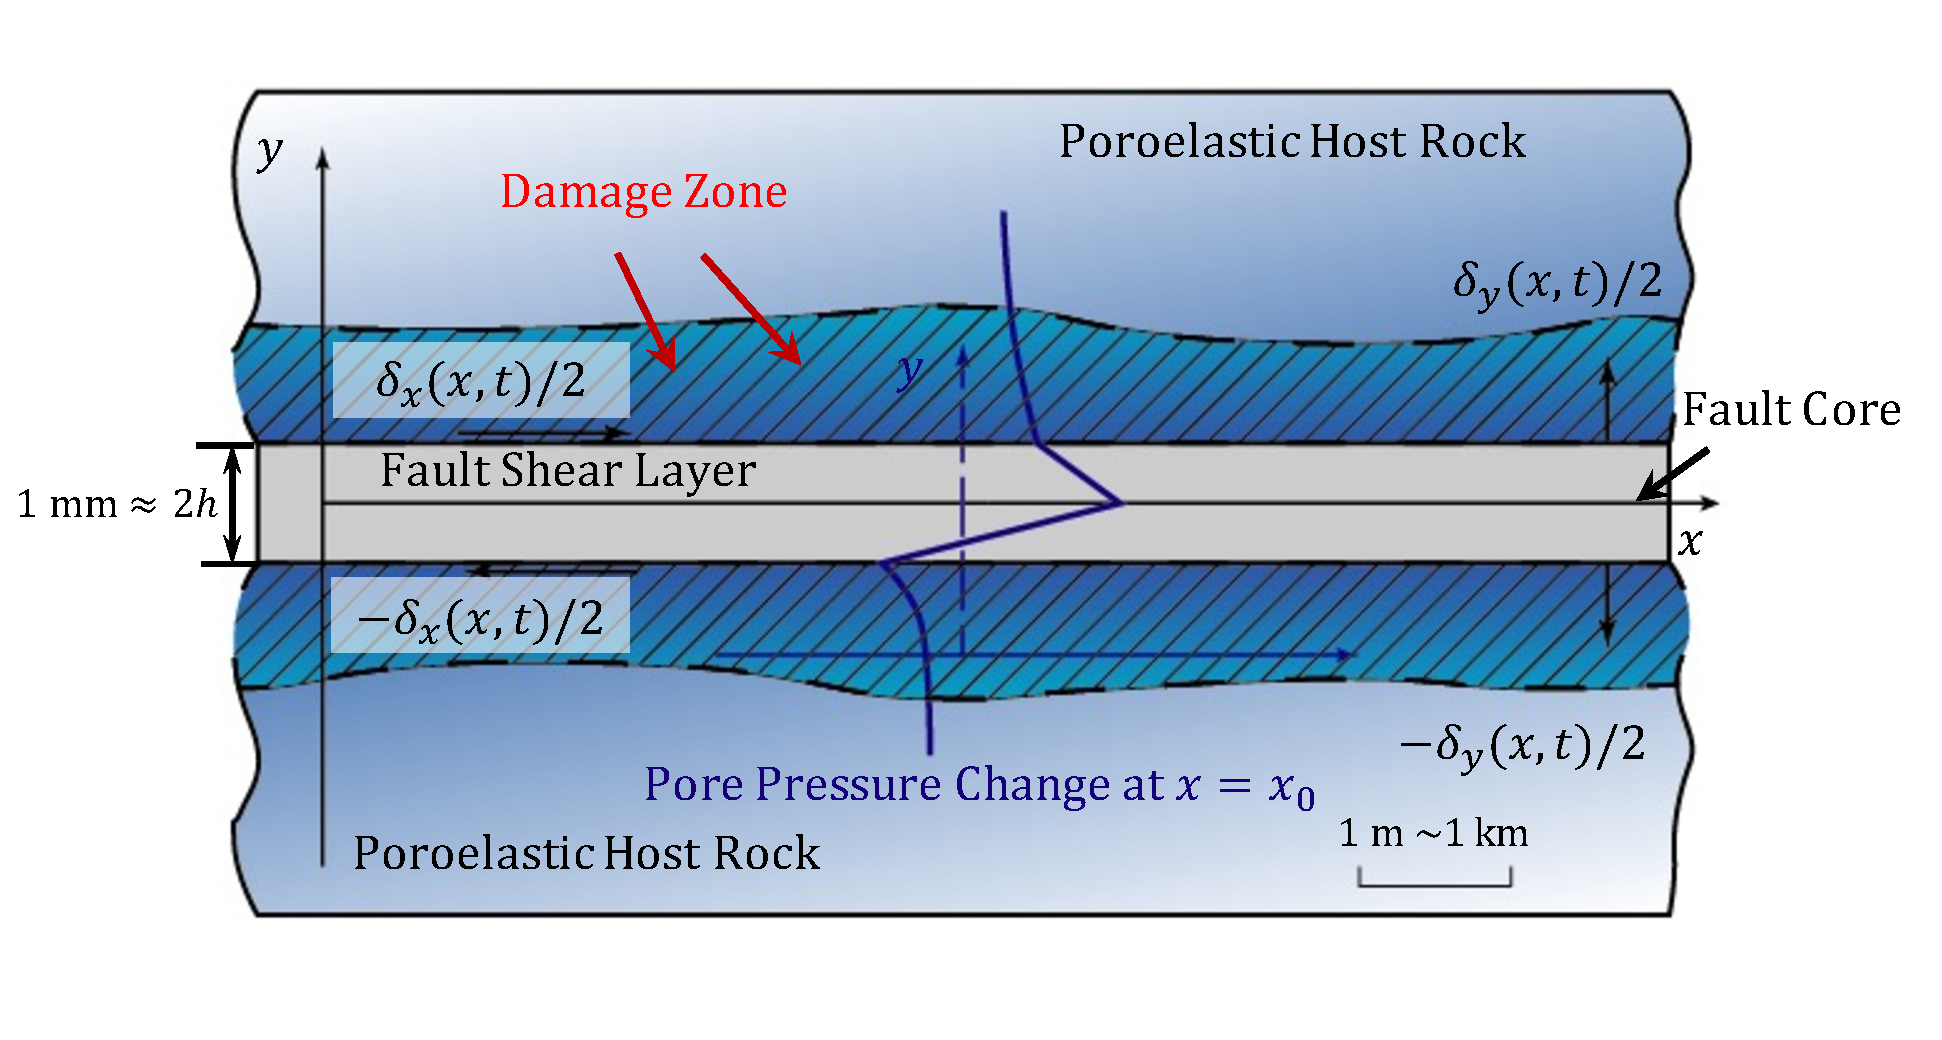
\includegraphics[width=1.0\textwidth]{final4.pdf}
    \caption{Model of pre-existing fault with poroelasticity, dilatancy, and damage zone.}
    \label{fig:conclusion 1}
\end{figure}

For example, Larochelle et al (2021) \cite{Larochelle_2021} studied fault slip under fluid injection using such a model supplemented with the along-interface fluid diffusion within the fault shear layer with a constant diffusivity.  The goal was to reproduce the results of a unique field experiment (Guglielmi et al., 2015 \cite{guglielmi_seismicity_2015}) and to examine the previously published conclusion (Bhattacharya et al., 2019 \cite{bhattacharya_induced_2019}) that the experimental data can only be explained by a model in which slow slip outruns the section of the fault pressurized by fluids.  
The study showed that a range of fault models can reproduce the outcomes of the field experiment, and the ones with higher reference friction (supported by laboratory studies) have slow slip well confined within the pressurized fault region, with important implications for fault stability and induced seismicity.   
While an advance over some previous studies of slip along pre-existing faults due to fluid injection, the modeling like in Larochelle et al. (2021) \cite{Larochelle_2021} is still significantly simplified. 

% Our goal is to build numerical models of sliding on pre-existing faults that more fully couple effects of fluids and nonlinear frictional fault slip, and validate those models through comparison with unique field and lab experiments. The important additional factors we would like to include are fluid pressure evolution due to inelastic shear dilatancy/compaction of the shearing layer, poroelasticity of the rock media, and changing poroelastic properties due to evolving off-fault damage (Figure~\ref{fig:future 2}). Inelastic dilatancy changes porosity, causing shear-induced evolution in pore fluid pressure within the layer; in part,  it can stabilize the fault slip acceleration by reducing the fault zone pore pressure \cite{segall_dilatancy_1995, Segall2010}. Poroelasticity causes changes in pore fluid pressure around the propagating shear rupture tip, since shear ruptures induce additional compressional and dilatational fields on the two sides of the fault, acting like a bi-material effect and inducing fluid flow across the shear layer and changes in the effective normal stress for the layer.  In part, these effects can destabilize fault slip in frictionally stable faults \cite{Heimisson2019}.  Off-fault damage changes permeability of the rock media \cite{faulkner_stuck_2011},with increases during slip events and healing in the inter-event period, as well as affects elastic properties and hence wave propagation \cite{Hudson1981}.  

While there are several numerical approaches for simulations of fluid flow in bulk rocks (e.g., Hart and Detournay, 1999 \cite{detournay_flac_1999}; Beljadid et al. \cite{Beljadid2020}, 2020; Cueto-Felgueroso et al., 2020 \cite{CuetoFelgueroso2020}), they typically do not include slip on well-developed pre-existing faults that can occur both quasi-statically and dynamically (with inertial effects, as during earthquakes). Developing such coupled numerical approaches is the goal of this work. The developed numerical approaches will be used to model field and lab experiments (e.g. Guglielmi et al., 2015 \cite{guglielmi_seismicity_2015}) as well as applied to induced seismicity and tectonic earthquakes. 